\documentclass[../main.tex]{subfiles}

\begin{document}
\section*{\centering 2. Stem - Functions}
	Identify the stem in the given image and explain its functions.\\[6pt]
	\rotatebox{90}{\large stem}
    \fcolorbox{red}{white}{
		\begin{minipage}{\dimexpr\textwidth-15\fboxsep-4\fboxrule\relax}
			
				Draw the direction of flow of nutrients in the stem and mark the parts of the stem. \\
				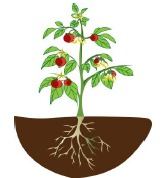
\includegraphics[width=6cm]{Task 5/images/plant.jpg} \\
				\\
				The stem transports \adash{1cm}\ and \adash{1cm}\ absorbed from the root. These nutrients move \adash{1cm}\ (Upwards/Downwards). \\
				The stem transports \adash{1cm}\ from the leaves. This nutrient moves \adash{1cm}\ (Upwards/Downwards). \\
			
		\end{minipage}
	}
	

\end{document}